\documentclass[a4paper,10pt]{article}
%\documentclass[a4paper,10pt]{scrartcl}

\usepackage[utf8]{inputenc}
\usepackage{graphicx}
\usepackage{listing}
\title{Cybersecurity\\
	Lab-report
}
\author{Moritz Rupp}
\date{Sommersemester 2022}

\pdfinfo{%
  /Title    ()
  /Author   ()
  /Creator  ()
  /Producer ()
  /Subject  ()
  /Keywords ()
}

\begin{document}
\maketitle
\newpage
\tableofcontents
\newpage
\section{Übung 1}
\textbf{A)}
Kali-IP:\\
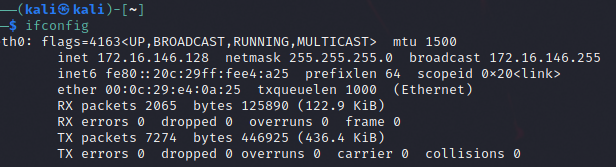
\includegraphics[scale=0.5]{kaliip.png}
\vspace{5mm}\\
\noindent Mit dem Nmap scan: \$ nmap -O 172.16.146.128/24 wird das Subnetzt mit OS detection gescannt.  Es werden unter anderem 5 Geräte gefunden. Eines davon zeigt als OS den Linux kernel an, was auf die Metasploitable VM hinweißt.\\
IP: 172.16.146.130\\
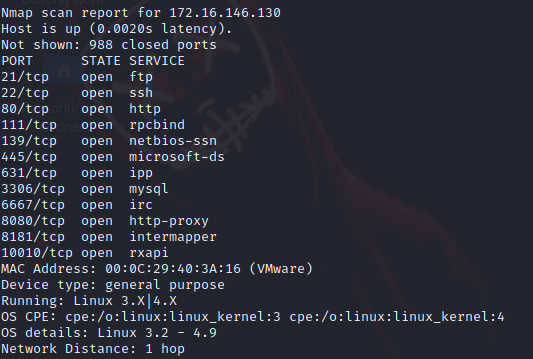
\includegraphics[scale=0.5]{nmapscan.png}\\
\textbf{B}

\noindent 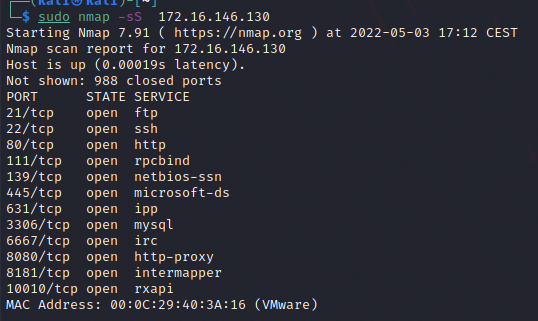
\includegraphics[scale=0.5]{nmapmeta.png}\\

\subsection{C}
Siehe A. Linux 3.2 - 4.9
\subsection{D}
\$ nmap -A 172.16.146.130
\\
\begin{verbatim}
 

21/tcp    open  ftp         ProFTPD 1.3.5
22/tcp    open  ssh         OpenSSH 6.6.1p1 Ubuntu 2ubuntu2.10 (Ubuntu Linux;2.0)
80/tcp    open  http        Apache httpd 2.4.7 ((Ubuntu))
|_http-server-header: Apache/2.4.7 (Ubuntu)
111/tcp   open  rpcbind     2-4 (RPC #100000)
139/tcp   open  netbios-ssn Samba smbd 3.X - 4.X (workgroup: WORKGROUP)
445/tcp   open  netbios-ssn Samba smbd 4.3.11-Ubuntu (workgroup: WORKGROUP)
631/tcp   open  ipp         CUPS 1.7
3306/tcp  open  mysql       MySQL (unauthorized)
6667/tcp  open  irc         UnrealIRCd
8080/tcp  open  http        Jetty 8.1.7.v20120910
8181/tcp  open  http        WEBrick httpd 1.3.1 (Ruby 2.3.7 (2018-03-28))
10010/tcp open  rxapi?

\end{verbatim}


\end{document}
